%appendixprefix sorgt dafür, dass "Anhang" vor jedem Anhang steht
%openany sorgt dafür, dass ein Kapitel auf jeder Seite beginnen kann
%        nicht nur rechts
%bibtotoc sorgt dafür, dass das Literaturverzeichnis automatisch im
%         Inhaltsverzeichnis erscheint
\documentclass[fontsize=11pt,paper=a4,parskip=half,draft=false,appendixprefix,bibliography=totoc,
headings=normal]{scrbook}


%
% neues if definieren, um zwischen PDF und DVI entscheiden zu können.
%
%\newif\ifpdf
%\ifx\pdfoutput\undefined
%\pdffalse %not PDFLaTeX
%\else
%\pdfoutput=1
%\pdftrue
%\fi
%\tracingstats=2
%\usepackage{layout}
% german language support (hyphenation etc)  
%\usepackage{ngerman}
\usepackage[ngerman]{babel}
% support for latin1 characters. That means you can enter ä ö ü ß directly
% no need for "a "u "ü "s anymore
%\usepackage[latin1]{inputenc}
\usepackage[utf8]{inputenc}
% provides the \url{} command to pretty print urls
\usepackage{url}

% needed for a german bibliography-style (s. below)
\usepackage[german]{babelbib}

% allows text flowing around figures.
\usepackage{wrapfig}

% allows to \includegraphics
\usepackage{graphicx}

% defines some standard colornames like "black" etc.
\usepackage{color}

% allows to color tablecells
\usepackage{colortbl}

% provides an easier interface to if-then-else constructs in 
% custom macros
\usepackage{ifthen}

% allows tables to break over pages.
\usepackage{supertabular}

% allows to have different kinds paper orientations in the same pdf-documnent
\usepackage{pdflscape}

% allows to specify absolute texpos for textboxes. This is generally only important for the titlepage
\usepackage[absolute]{textpos}

% allows to enumerate different figures with a) b) in the same figure-environment.
\usepackage{subfigure}

% finetune the gaps between figure and text in the subfigure environment (basically close the gap as much as possible)
\renewcommand{\subfigtopskip}{0pt}
\renewcommand{\subfigbottomskip}{0pt}

% some color definitions for the pdf-statements below
\definecolor{mygrey}{rgb}{0.45,0.45,0.45}
\definecolor{mydarkgrey}{rgb}{0.2,0.2,0.2}
\definecolor{red}{rgb}{1.0,0.33,0.33}
\definecolor{orange}{rgb}{1.00,0.73,0.33}
\definecolor{yellow}{rgb}{0.95,0.92,0.}
\definecolor{lightgreen}{rgb}{0.3,0.95,0.46}
\definecolor{titleblue}{rgb}{0.03,0.10,0.46}

%\ifpdf
% Metadata and configuration of the pdf output:
% Do not forget to enter the correct title, author, subject und keywords

% For screen viewing it is nice to have references marked in a slightly different
% color than the rest of the text. Since they will be hyperlinks to the 
% referenced objects.
\usepackage[pdftex,
             pdftitle={Erweiterung des CT Game Studios um einen "Open Stage" Modus},
             colorlinks,
%             linkcolor={mydarkgrey},
%             citecolor={mygrey},
%             urlcolor={black}
             linkcolor={lightgreen},
             citecolor={mygrey},
             urlcolor={blue},
             plainpages={false},
             bookmarksnumbered={true},
             pdfauthor={Daniel Rose},
             pdfsubject={},
             pdfkeywords={},
             pdfstartview={FitBH}]{hyperref}

% For the final printouts (remember - you need at least three - one for each examiner and one for the archive 
% [ This might have changed - so contact the "Prüfungsamt" about the current regulations !! ] - it is better
% to have all text in the same color (namely black).
% 
%\usepackage[pdftex,
%            pdftitle={},
%            colorlinks,
%            linkcolor={black},
%            citecolor={black},
%            urlcolor={black},
%            plainpages={false},
%            bookmarksnumbered={true},
%            pdfauthor={},
%            pdfsubject={},
%            pdfkeywords={},
%            pdfstartview={FitBH}]{hyperref}
\pdfcompresslevel=9
%\fi

% some configuration for the amount of text on a single page
\usepackage{typearea}\areaset[1.5cm]{418pt}{658pt}
\setlength{\headheight}{37pt}

% To avoid nasty mistakes like having comments directly in the textflow
% the following \todo macro was defined. With that you can enter
% \todo{What I still have to do here} 
% inside of your text and a marker will appear at the page's margin with the 
% text "What I still have to do here".
% The first line activates this feature. If you comment it out and uncomment
% the second line below there will be no error messages and no todos will be show
% anymore. So - even if you have forgotten to delete one of them - they will not appear
% in the final printout. 
\newcommand{\todo}[1]{\marginpar{\textcolor{red}{ToDo:} #1}}
%\newcommand{\todo}[1]{}

% We recommend to split your document into several files. Usually one for every chapter is a 
% good idea. If you follow this guideline (how to assemble these files in a single document
% see two paragraphs below) you will be able to single out chapters via the \includeonly{}
% command. Using this mechanism page numbering and references of the full run before will be
% preserved. This also nice, if your latex run tends to get slow and you need to fine tune 
% some formatting in one chapter - just include that one. The rest (or at least the ones before
% the one currently under construction) will remain untouched. This means a boost in compilation time.
%\includeonly{chapter2}



%\usepackage[style=authoryear-ibid]{biblatex}
\usepackage[german=quotes]{csquotes}

%\bibliography{references}

\begin{document}
% the next two lines influence the detailedness of the table of contents
% and to what structure depth numbers are written before sections/subsections/paragraphs
% You should not touch this
\setcounter{tocdepth}{3}
\setcounter{secnumdepth}{3}
\frontmatter
% here the titlepage is included. Look into the file "titelseite.tex" to 
% adapt it to your needs (name, title etc.)
% Titelseite braucht folgenden  Eintrag
% \usepackage[absolute]{textpos}
% textpos ist nicht Bestandteil von tetex
% kann aber von dante heruntergeladen werden
\begin{titlepage}
\vspace*{-1cm}
\newlength{\links}
\setlength{\links}{0.9cm}
\setlength{\TPHorizModule}{1cm}
\setlength{\TPVertModule}{1cm}
\textblockorigin{0pt}{0pt}

\sffamily
\LARGE

\begin{textblock}{16.5}(2.8,2.6)
 \hspace*{-0.25cm} \textbf{UNIVERSITÄT DUISBURG-ESSEN} \\
 \hspace*{-1.15cm} \rule{5mm}{5mm} \hspace*{0.05cm} FAKULTÄT FÜR INGENIEURWISSENSCHAFTEN\\
 \large{}ABTEILUNG INFORMATIK UND ANGEWANDTE KOGNITIONSWISSENSCHAFT\\
\end{textblock}


%Hier Titel, Name, und Matrikelnummer eintragen, \\ make a newline
\begin{textblock}{14.5}(3.2,8.5)
  \large
{ \textbf{Bachelorarbeit}} \\[1cm]
{\LARGE \Large\textbf{Erweiterung des CT Game Studios um einen \enquote{Open Stage} Modus}} \\[1.3cm]
Daniel Rose\\
Matrikelnummer: 2270435
\end{textblock}



\begin{textblock}{10}(10.5,17.5)

\includegraphics[scale=1.0]{unilogo.pdf}\\
\normalsize
\raggedleft
Abteilung Informatik und angewandte Kognitionswissenschaft \\
Fakultät für Ingenieurwissenschaften \\
Universität Duisburg-Essen \\[2ex]

\today\\[15ex]
\raggedright
% Supervisors
{\textbf Betreuer:} \\
Prof. Dr. H.~U.~Hoppe\\
Sven Manske\\
Sören Werneburg\\
\end{textblock}

\end{titlepage}

\tableofcontents
\listoffigures
\mainmatter

% To assemble the whole document
% Please be aware that each file will begin on a new page
% therefore chapters should be put into such a file.
% There cannot be an include statement inside of an "included" file.
% So if you want to further divide your document - use \input inside of 
% the included files. \input will not begin on a new page.
\chapter{Einleitung}

\section{Motivation}

Computer betreffen jedes Leben und haben großes Potential und Herausforderungen -> Mündige Bürger
sollten Computer programmieren können -> CT Skills -> auch hilfreich im Alltag und Job

Spiele haben sich als effektive Lernumgebungen heraus gestellt -> CT in Spiel vermitteln


Welche Spiel-Aspekte sind wichtig um Lernfortschritt zu erzielen? Wie lässt sich das Spiel in
den Unterrichtsalltag einbinden?


"Wie Facebook 4 Mio. Datensätze verloren hat" (Fakenews 2017). "AI wird uns zerstören" (Fakemag,
2015). "Big Technology invests 500 M to bring CS into schools" (Mustermag, 2017). Die Informatik
umgibt nahezu alle Menschen, sie transformiert unseren Alltag und unseren Arbeitsplatz. Dies
erfordert eine Gesellschaft, die in Kontrolle der Technologie ist, und weiß, wie damit umzugehen
ist. Dabei fangen wir gerade erst an, die Informatik auch in dieser Reichweite und angemessenen
Umfang in die Schulen zu bringen.

Mit "Computational Thinking" hat Jeanette Wing einen einflussreichen Forschungsansatz gestellt zu
der Frage "Welche Fähigkeiten werden in der Informatik gebraucht?". Unter diesem Begriff haben sich
eine Reihe von Curricula und Werkzeugen gesammelt, die versuchen, diese Fähigkeiten Schülern und
anderen Interessierten näher zu bringen.

Mit RoboPlanet wurde ein Spiel entwickelt, bei dem der Lernende mittels einem zugänglichen visuellen
Programmiersprache einen Roboter programmiert, um verschiedene Spielziele zu erreichen. Das Spiel
besitzt einen Storymodus, bei dem dem Spieler schrittweise neue Programmierkonzepte beigebracht
werden. Zu Ende der Story kann der Roboter komplexe Probleme lösen.

Während der Lernende mit dem Storymodus eine geleitete

\section{Aufgabenstellung}

Im Rahmen dieser Arbeit wird RoboPlanet um einen offenen Spielmodus erweitert, bei dem der Spieler
seinen Roboter gegen andere Roboter antreten lässt. Im Training entwickelt der Schüler Strategien,
um die Gegner, die wiederrum verschiedene Kampfstrategien besitzen, zu besiegen. In einem
klassenübergreifenden Wettbewerb werden die entwickelten Roboter gegeneinander antreten. Durch die
Erweiterung soll motiviert werden, und fortgeschrittene, nahezu unbegrenzte Programmierung gefördert
werden.


\section{Aufbau der Arbeit}

Im Folgenden wird zunächst dargestellt, wie Computational Thinking durch RoboPlanet gefördert wird.
Dazu wird die Theorie und verwandte Arbeiten vorgestellt. Wir untersuchen die Bestandteile von
Computational Thinking, und die Mechanismen mit denen Schüler diese Bestandteile lernen, bzw. Lernen
dieser Bestandteile gefördert werden. Daraufhin wird exploriert, welchen Mehrwert RoboArena bringt,
welche Konzeption daraus entsteht, und wie dieses technisch umgesetzt wird.

Test \cite{Ikeda1997}


\chapter{Grundlagen}

\section{Computational Thinking}

Unter Computational Thinking (CT) wird Kognitionsprozess oder Gedankenprozess verstanden, der durch
die Fähigkeit, in Form von Dekomposition, abstrahierend, evaluierend, algorithmisch und
generalisierend zu denken, reflektiert wird \cite{selby_computational}. Nach \cite{wing2011research}
ist Ziel des Prozesses, ein Problem so darzustellen, dass es von einem Computer gelöst werden kann.  
Dazu werden zur Entwicklung von Problemlösungen logische Artefakte erstellt, die auf dem Computer
ausgeführt werden. Dies kann zum Beispiel Quelltext in einer Programmiersprache sein.

Diese Arbeit fokussiert sich primär auf algorithmisches Denken, Abstraktionen und Evaluation.
Algorithmisches Denken beschreibt die Fähigkeit, ein Problem sequentiell abzuarbeiten. Dazu werden
Kontrollstrukturen als Teil eines Abstraktionsprozesses genutzt. Um zum Beispiel eine Wiederholung
eines Befehls umsetzen, könnte der Befehl mehrfach hintereinander im Quellcode stehen. Zur
Komprimierung des Codes kann man die Wiederholung mit einer Schleife abstrahiert werden. Dazu muss
ein zusätzliches Vokabular verwendet werden, dass dem Computer klar macht, dass dieser Befehl
mehrfach wiederholt werden soll. Eine tiefere Abstraktion kann an diesem Beispiel erfolgen, wenn
durch die Nutzung von Variablen innerhalb der Schleife mit jeder Wiederholung unterschiedliche Werte
benutzt werden. Ein weiteres abstrahierendes Konzept besteht darin Prozeduren und Funktionen zu
bilden. Dabei werden mehrere Kommandos werden unter einem Namen gebündelt und parametrisiert, und im
Fall von Funktionen ein Rückgabewert generiert. Prozeduren und Funktionen können mehrmals an
verschiedenen Stellen im Programm aufgerufen werden zu können, ohne die Kommandos einzeln zu
wiederholen. Abstraktionen erlauben uns Konzepte auf einer Metaebene zu nutzen und diese dann
umzusetzen.

Zur Entwicklung der logischen Artefakte gehört neben der Programmierung selbst auch die Evaluation
des Artefakts. Dazu wird es ausgeführt und anschließend mithilfe von visuellen oder textuellen
Feedback analysiert. Aufgrund des Feedbacks werden Rückschlüsse darüber gezogen, ob das zugrunde
liegende Problem gelöst wurde, und wenn nicht, wie das Artefakt verändert werden muss, um das
Problem adäquat zu lösen.

In einer Richtlinie zur Etablierung von Computational Thinking in der K-12-Bildung
(\cite{leadership_toolkit}) der International Society for Technology in Education und Computer
Science Teacher Association wird die Wichtigkeit von CT beschrieben: \em \enquote{Because we can
expect that every student will rely on computing in some way to amplify his or her skills, we must
ensure that all students have the opportunity to learn the basics of CT during their K–12
education.} \em.

\section{Turtle Geometrie}

Den Computer als Werkzeug zum Lernen zu benutzen ist der Fokus von Seymour Paperts Forschung zu Logo
und der Turtle-Umgebung \cite{papert1980mindstorms}. Logo ist eine Programmiersprache die dazu
gestaltet ist, möglichst einfach zu erlernen zu sein. Dazu besitzt sie eine minimale Syntax und ein
minimales Kontingent an Kontrollstrukturen.

Papert konzipiert die Turtle-Umgebung zur Exploration mathematischer Konzepte. Sie ist ein Beispiel
einer Mikrowelt, eine Anwendung in der Objekte programmatisch manipuliert werden können, um dem
Lerner ein Medium zu bieten, dass dem natürlichen Erlernen eines Konzepts dient. Die Turtle ist ein
Objekt, das mithilfe von einfachen Kommandos bewegt werden kann. Durch Aktivierung eines Stifts wird
die Ausgabe von Linien erzeugt, die der Bewegung folgen. Die Bewegung der Turtle erfolgt mittels
Logo-Programmen.

Papert argumentiert, dass eine Mikrowelt dann zum einem wertvollen Lerninstrument wird, wenn sie dem
eine natürliche Interaktion erlaubt. Die Bewegung der Turtle soll dem Sprechen mit der Turtle
gleichen. Die Definition von Prozeduren gleicht dem Beibringen eines neuen Vokabulars. Das Erlenen
eines Konzepts wird dann durch iteratives Vorgehen ermöglicht, dass der Exploration und dem Lernen
einer der menschlichen Sprache im Kindesalter gleicht. Das Objekt, dass in der Mikrowelt manipuliert
wird, sollte dabei menschliche Charakteristiken besitzen. Die Turtle ist \enquote{body-syntonic},
ihre Bewegung und Orientierung lässt sich konkret auf die Bewegung und Orientierung des Menschen
übertragen. Um das Verhalten der Turtle nachzuvollziehen, kann der Lerner den eigenen Körper als
Referenz nutzen.


\section{Game-based learning von Computational Thinking}

Spiele werden häufig dazu genutzt, als Lernumgebungen zum Erlenen von Computational
Thinking-Konzepten zu dienen (z.B. \enquote{Program your Robot} \cite{kazimoglu_serious_2012},
\enquote{Lightbot} \cite{gouws2013computational} oder AgentSheets \cite{repenning2010scalable}). Diese Lernumgebungen zeichnen sich dadurch aus, dass sie Computational Thinking-Fähigkeiten direkt auf Spielelemente mappen. Zusätzlich können Spiele aufgrund der Herausforderung, die sie stellen, einem Fantasieaspekt der den Lerner in
eine imaginäre Welt versetzt, dem Ausnutzen der natürlichen menschlichen Neugierde, und der
Kontrolle, die der Lernen über den Spielverlauf zu geben, Mikrowelten in einer Weise bereit stellen,
in der Lerner internal motiviert sind Spielziele zu verfolgen und damit Lernerfolge zu erzielen
(\cite{rieber_seriously_1996}).

\subsection{RoboCode}

RoboCode\footnote{https://sourceforge.net/projects/robocode/} ist ein Spiel, dass zum Erlernen der
Programmiersprache Java konzipiert wurde. In einer Arena (Abb. \ref{robocode}) versuchen zwei oder mehrere Roboter sich
gegenseitig zu zerstören. Dabei führen die Roboter Kampfstrategien in Form von Java-Programmen aus.
RoboCode integriert einen Quellcode-Editor, in dem diese Strategien gebaut werden können.
Mitgelieferte Beispielstrategien können als Orientierung dienen und als Gegnerstrategien festgelegt
werden.

\begin{figure}
  \caption{Ein Kampf zwischen zwei Robotern in RoboCode.}

  \label{robocode}
  
  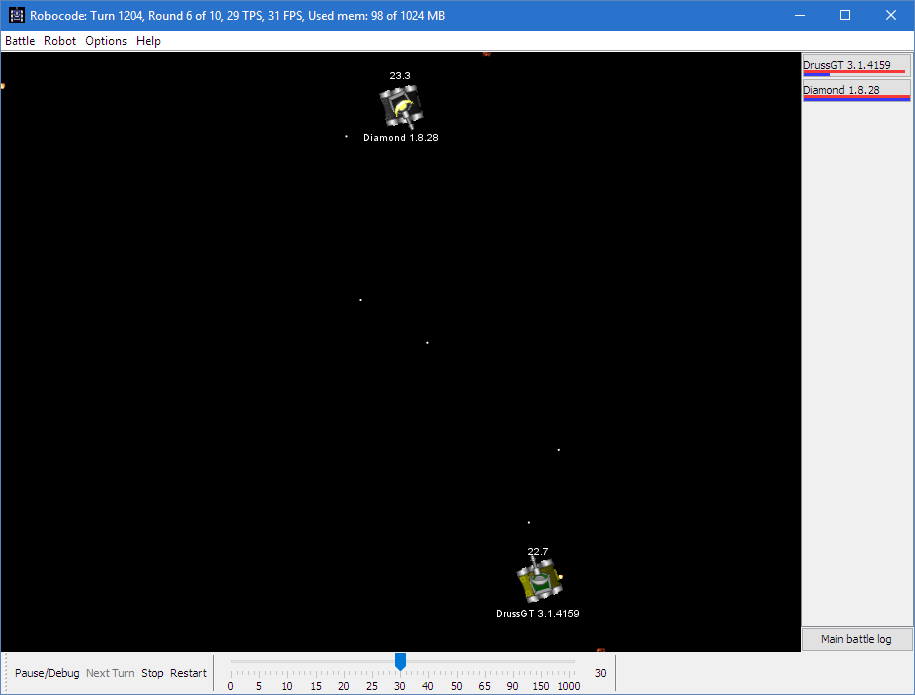
\includegraphics{figures/RoboCode.png}
\end{figure}

Um RoboCode hat sich eine Community gebildet. Im
RoboCode-Wiki\footnote{http://www.robowiki.net/wiki/Robocode} enthält eine Dokumentation des Spiels,
Anleitungen zum Erstellen eigener Strategien, und weitere Kampfstrategien zum Download.
RoboRumble\footnote{http://literumble.appspot.com/} ist eine Sammlung von dauerhaft aktualisierenden
Ranglisten, in denen von Spielern hochgeladenene Kampfstrategien aufgrund von Kämpfen gegeneinander
eingestuft werden. Die Strategien können heruntergeladen, eingesehen und für eigene Kämpfe benutzt
werden.

\subsection{ctGameStudio}

CTGameStudio (\cite{werneburg_ctgamestudiogame-based_2018}) ist eine webbasierte Spielumgebung zum
Erlernen von CT-Fähigkeiten und Programmierung. Mithilfe eines Editors entwickeln Schüler ein
Programm zur Steuerung eines virtuellen Roboters in einer Mikrowelt.

Der Editor ist ein visuelles, blockbasiertes Programmierwerkzeug basierend auf der
Blockly-Bibliothek\footnote{https://developers.google.com/blockly/}. Visuelle blockbasierte Editoren
haben sich als einsteigerfreundliche Programmierwerkzeuge erwiesen (\cite{weintrop_block_2015}).
Programmkonstrukte werden durch Blöcke repräsentiert, die mittels Drag-and-Drop ineinander
verschachtelt und kombiniert werden, um ein Programm zu bilden. Eine Blockbibliothek gibt eine
eingebaute Übersicht über die verfügbaren Programmkonstrukte, so dass auf einen Blick die
Möglichkeiten der Programmierung eingesehen werden können. Durch die strukturierte Komposition von
Blöcken können keine Syntaxfehler auftreten, was in textbasierten Programmen eine häufige, den
Spielfluss störende Fehlerquelle ist.

Zur Einführung in die Programmierung und Vermittlung von CT-Fähigkeiten, sowie zur Einführung in die
Mechaniken des Spiels enthält das ctGameStudio einen Storymodus. Der Storymodus enthält mehrere
Level, die nacheinander abgearbeitet werden, und jeweils auf das Erlenen einer oder mehreren
CT-Fähigkeiten, einer neuen Abstraktion oder Roboterfähigkeit abzielen. Dazu enthält das Level eine
Aufgabenbeschreibung, Anleitungen und optionale Hilfestellungen. Zur Lösung eines Levels baut der Schüler ein
Programm welches einen Algorithmus darstellt, der den Roboter so steuert, dass die Herausforderung
gelöst wrid. Diese Problemlösungstrategie kann immer wieder neu ausgeführt werden, bis das
gewünschte Ziel erreicht wurde. Ist das der Fall, wird zum nächsten Level fortgeschritten. Mit
steigenden Level erhöht sich die Komplexität der benötigten Lösungstrategien. So reicht im ersten
Level ein einfacher Befehlsaufruf, während im letzen Level durch gezielte Bewegung, Zielen und
Schießen ein Gegner besiegt werden, bevor dieser einem zu viel Schaden zufügt.

Angelehnt an der Turtle-Geometrie nach Papert wurde eine Bewegungssemantik für den Roboter
entwickelt, und um Fähigkeiten erweitert, die für die das Spielen der Story relevant sind.

\begin{itemize}
\item Positionierung auf dem Spielfeld durch die Bewegung um eine Distanz oder bis zu einem Punkt
auf der x- und y-Achse, der Bewegung bis die Spielfeldgrenze, ein Gegenstand oder der Gegner berührt wurde, dem Drehen um einen
Winkel, und dem Drehen, um einen Punkt anzupeilen.
\item Angriff durch Abgeben eines Schusses in Blickrichtung.
\item Das Ausfinden machen des nächstgelegenden Objektes oder Gegners durch einen Scanvorgang in eine Richtung. Wurde
  ein Ergebnis gefunden, kann die Distanz und Winkel zum Ergebnis und seine Position gelesen werden.
\item Feststellen von Ereignissen, wie der Fall ob man getroffen wurde, oder ob man mit der Wand,
  einem Gegner oder einem Objekt kollidiert ist.
\item Lesen der eigenen Attribute, darunter die Position auf dem Spielfeld und die Anzahl an
verbleibenden Lebenspunkten.
\end{itemize}

Nach Beenden des letzten Levels sind die Inhalte des ctGameStudio im aktuellen Stand ausgeschöpft.
Dabei wäre es sinnvoll, Schülern eine Möglichkeit zu geben, ihre gelernten Fähigkeiten anzuwenden.
Während Schüler im Storymodus konkrete Anweisungen zu der Lösung eines Problems bekommen, sollte das
Spiel Herausforderungen enthalten, die eigenständig vom Schüler gelöst werden müssen, um besonders
die Evaluationsfähigkeit stärker auszubilden. Spiele wie RoboCode zeigen uns, dass ein Spiel durch
einen offenen Spielmodus einen hoher Wiederspielwert erreicht werden kann.

\chapter{Ansatz}

Im Storymodus des ctGameStudios lernen Schüler grundlegende Konzepte der Programmierung wie
Schleifen, Verzweigungen, Ereignisse, Prozeduren und Funktionen kennen. Der Storymodus ist in sich
geschlossen, da er einen festen Anfang und Ende hat, und im vornherein festgelegte, spezifische
Herausforderungen stellt.

Wir wollen das ctGameStudio erweitern, um Spielern die Möglichkeit und die Motivation dazu zu geben,
die im Storymodus gelernten Fähigkeiten anzuwenden und zu trainieren. Im Gegensatz zum Storymodus
soll dieser Spielmodus offen sein, so dass der Spieler seine Herausforderungen und Lösungsansätze
selbst bestimmen kann. Damit wiederholtes Spielen motiviert wird und die eigene Kreativiät gefördert
wird, sollen Herausforderungen durch sich selbst oder andere generiert werden können. 

Ein offener Spielmodus stellt die Fähigkeit in den Vordergrund, Problemstellungen zu analysieren,
und adäquate Problemlösestrategien zu entwickeln. Dadurch werden speziell die CT-Fähigkeiten der
Abstraktion und der Evaluation gefördert.

Inspiriert vom RoboCode und angelehnt an das letzte Level des Storymodus soll dieser Spielmodus aus
einem Roboterkampf bestehen. Es gilt, eine Strategie zu entwickeln, um die Strategie des Gegners zu
überwinden.

\section{Ein Lernszenario}

Das Spiel soll solche Schüler unterstützen, die die Grundlagen der Programmierung kennen lernen und
ausbauen sollen. Der Kernlehrplan Informatik für Gymnasien und Gesamtschule in der Sekundarstufe II
(\cite{SchulministeriumNRW2014}) definiert als Inhaltsfeld die Entwicklung von Algorithmen, welche
als "genaue Beschreibung zur Lösung eines Problems" (S. 17) definiert werden. Dies entspricht
der Entwicklung von Problemlösestrategien in der Roboter-Mikrowelt des ctGameStudio, und zeigt, dass
das dieses Spiel die Anwendung in der Sekundarstufe II unterstützen sollte.

Folgendes Lernszenario soll darstellen, wie das Spiel die Ziele des Lehrplans unterstützt und in den
Unterricht eingebunden werden kann.

Um die Grundlagen des Spiels sowie die zur Entwicklung von Problemlösestrategien nötigen
Programmierkonzepte kennen zu lernen, spielen Schüler zunächst den Storymodus des ctGameStudio.
Durch Bearbeiten der Level des Storymodus werden die im Kernlehrplan definierten inhaltlichen
Schwerpunkte der Analyse, Entwurf und Implementierung einfacher Algorithmen (S. 23) unterstützt, und
anhand dessen die Kompetenzen des Argumentierens, der Modellierung, der Implementation, des
Darstellen und Interpretieren und Kommunizieren und Kooperieren gefördert.

Mit dem offenen Spielmodus werden die erlenten Kompetenzen vertieft. In Kämpfen zwischen dem eigenen
gegen einen Gegnerroboter entwickeln die Schüler eigene Kampfstrategien. Dabei können sie die
Gegnerstrategie aus eigenen oder vorgefertigten Strategien festlegen, um eine generell anwendbare,
gegen viele Herausforderungen effektive Strategie zu entwickeln. Nachdem die Schüler eine oder
mehrere Strategien entwickelt haben, kann der Lehrer ein Turnier veranstalten, in dem die Strategien
gegeneinander ausgespielt werden und eine Rangliste entsteht. Das Turnier wird an einem gemeinesamen
Bildschirm oder Projektion verfolgt, und liefert eine Diskussionsgrundlage um Strategien gemeinsam
zu evaluieren. In weiteren Durchgängen können Schüler ihre Strategie verbessern, und weitere
Turniere veranstaltet werden.


\section{Offener Spielmodus: RoboStrategist}

Kern des offenen Spielmodus ist der Kampf zwischen zwei Robotern, die vorprogrammierte Strategien
ausführen. Die Strategien sind Algorithmen zur Koordination der Fähigkeiten des Roboters, um den
Gegner Schaden zuzufügen, und eigenen Schaden zu vermeiden. Eine erfolgreiche Strategie besteht aus
effektiver Positionierung des Roboters auf dem Spielfeld, dem Ausweichen von Schüssen nachdem man
getroffen wurde, dem Ausfinding machen und Verfolgen des Gegners, und das Zielen und Schießen auf
den Gegner.


\subsection{Training}

Der Training fördert eigenständiges, selbst-geleitetes Lösen von Problemen, und bietet damit
eine Plattform, seine Programmierfähigkeiten zu vertiefen. Zum Einen werden komplexe
Herausforderungen in Form von unterschiedlichen Gegnerstrategien gestellt. Der Spieler
wendet Abstraktionen wie Schleifen, Verzweigungen, Variablen, Prozeduren und Funktionen an, um einen
Algorithmus zu entwickeln. Der Algorithmus ist das Code-Artefakt, das gegen das Problem in Form der 
Gegnerstrategie evaluiert wird.

Zum Anderen kann der Spieler eigenständig wählen, wie er bei der Entwicklung der
Problemlösestrategie vorgeht, in dem er selbst wählt, gegen welche Strategien er seine Strategie
testet. Im Rahmen dieser Arbeit sollen dafür dafür drei vorgefertigte Gegnerstrategien verfügbar
sein. Die Strategien unterscheiden sich in ihren Ansätzen, ihrer Komplexität, und der Schwierigkeit,
sie zu besiegen.

Die erste Strategie, \enquote{Verwirrt}, (Abb. \ref{strategie-verwirrt}) ist dazu gestaltet, einen
einfachen Einstieg in die Strategieentwicklung zu geben. Der Roboter bewegt sich in zufälligen
Zeitabständigen auf zufällig gewählte Positionen, und gibt zwischendurch Schüsse in zufällige
Richtungen ab. Um den Roboter zu besiegen, muss der Spieler eine Strategie entwickeln, die den
Gegner immer wieder auffindet, und Schüsse in seine Richtung feuert. Dadurch, dass kein
Zielen auf den Roboter des Spielers besteht, muss die Lösungsstrategie nicht besonders effizient
sein. Auch um die eigene Positionierung muss sich der Spieler keine Gedanken machen.

Die zweite Strategie, \enquote{Wandkrabbler} (Abb. \ref{strategie-wandkrabller}), agiert in einem
vorsehbaren Muster. Der Roboter bewegt sich an am Spielfeldrand entlang und scannt in kleinen
Abständen voneinander entgegengesetzt der Wand nach dem Gegner. Wurde dieser entdeckt, schießt er
solange, bis der Gegner seine Position ändert. Diese Strategie erfordert vom Spieler eine Strategie
zu entwickeln, in der unterschiedliche Postionen eingenommen werden, um die Entdeckung durch den
Gegner zu verzögern und im Fall eines Treffers weiteren Schüssen auszweichen. Die erhöhte Gefahr
durch den Wandkrabbler erfordert auch einen effizienten Scanvorgang, so dass man den Gegner öfter
und schneller auffindet und Schaden zufügt, als er es tut.

Die dritte Strategie, \enquote{Eckenschütze} (Abb. \ref{strategie-wandkrabller}), ist die
gefährlichste aller Strategien. Zunächst hat sie den effizientesten Scanmechanismus. Dazu bewegt der
Roboter sich zwischen den Ecken des Spielfelds, und scannt von den Ecken aus in kleinen Schritten
das gesamte Spielfeld ab. So ist die Chance groß, innerhalb eines kurzen Zeitraums den Gegner
aufzufinden. Wurde der Gegner entdeckt, werden so lange Schüsse abgegeben, bis der Gegner seine
Position ändert. Die Strategie implementiert zudem einen Ausweichmechanismus, so dass der Roboter in die
nächste Ecke wechselt, wenn er getroffen wurde. Um diese Strategie zu besiegen erfordert ständige
Bewegung auf dem Spielfeld, um den Scanvorgängen zu entgehen. Wahrscheinlich sollte sie ein eigenen
Ausweichmechanimus implementieren, und einen effiziente Scanvorgang beinhalten.

Wie bereits vorgestellt sollte eine Mikrowelt nach Papert ein iteratives, selbst gesteuertes Vorgehen
erlauben, um die inherente Kreativität und Explorationswillen des Menschen zu nutzen. In diesem
Sinne wollen wir dem Spieler die Möglichkeit geben, als Gegnerstrategien neben den vorgefertigten
auch selbst erstellte Strategien zu wählen. Um seine Strategie zu verbessern, könnte der Spieler
durch eine Analyse Schwachpunkte seiner Strategie feststellen, und versuchen diese mit einer neuen
Strategie konkret auszunutzen.

Das eigenständige, selbst-geleitete Lösen von Problemen soll einen kreativen Lösungsprozess des
Spielers fordern, ein exploratives Vorgehen motivieren, und damit verglichem mit dem geleiteten
Prozess des Storymodus einen höheren Lerneffekt erzielen.

Folgendes Schema stellt eine neue Strategieentwicklung dar.
% und zeigt, dass die Entwicklung einer Strategie im Training den drei Stufen des Compuational Thinking Prozesses \ref{repenning_principles_2017}

\begin{enumerate}
\item Die initial geladenene Gegnerstrategie wird ausgeführt.
\item Man analysiert die Gegnerstrategie und bildet erste Lösungsansätze (Problem Formulation).
\item Man formuliert und implementiert erste Lösungsansätze (Solution Expression). Man kann auf das Wissen aus den letzten
Leveln des Storymodus zurückgreifen, um einen ersten Anhaltspunkt dafür zu haben.
\item Man führt den Kampf aus und analysiert seinen Verlauf (Solution Execution \& Evaluation). Die Evaluationskriterien sind, ob der Roboter
das macht, was man mit dem Programm erzielen wollte, und ob der Problemansatz zum Erfolg führt.
\item Aufgrund der Analyse verbessert der Spieler seine Strategie.
\item Schritt 4 und 5 werden wiederholt, bis der Gegner wiederholt geschlagen werden kann.
\item Der Spieler wählt eine neue Gegnerstrategie.
\item Schritt 4 bis 7 werden wiederholt, bis der Spieler alle Gegnerstrategien hat. Der Spieler kann außerdem
versuchen, seine eigene Strategie zu besiegen, in dem er sie als Gegnerstrategie festlegt.
\end{enumerate}

Um verschiedene Strategieansätze ausprobieren zu können, und in mehreren Sitzungen an den Strategien
arbeiten zu können, kann der Spieler seine Strategien speichern, kopieren, neue anlegen, und
zwischen diesen wechseln.


\subsection{Turniere}

Turniere sind spannend und erhöhen Spielspaß und damit die Motivation, das Spiel zu spielen. Der
kompetitive Aspekt wird Spieler dazu motivieren, gute Strategien zu entwickeln. Die
Turnierdurchführung selber bietet einen Vergleich zwischen Strategien und ist so
Diskussionsgrundlage für verschiedene Strategieansätze und Verbesserungen.

Da es verschiedene Möglichkeiten gibt, ein Turnier durchzuführen, und diese ihre eigenen Vor- und
Nachteile haben, wollen wir dem Turnierveranstalter die Wahl eines Turniersystems geben. In dieser
ersten Version des Open Stage-Modus wollen wir die zwei gebräuchlisten Turniersysteme zur Wahl
stellen.

Das Jeder-gegen-Jeden-System ist die ausführlichste Weise, ein Turnier durchzuführen. Ein Beispiel
für diese Turnierart ist die deutsche Fußballbundesliga. Um in diesem System eine Rangfolge zwischen
Teilnehmern zu erzielen, tritt jeder Teilnehmer gegen jeden anderen Teilnehmer an und zählt die
Siege, die erreicht wurden. Vorteil ist, dass diese Rangfolge erschöpfend ist. Nachteil dieses
Modus ist die quadratisch steigende Anzahl von Kämpfen ($n x n$ Kämpfe bei $n$ Teilnehmern),
die durchgeführt werden müssen. Für die Evaluation von Strategien im Open Stage-Modus bietet sich das
Jeder-gegen-Jeden-System an, wenn eine geringe Anzahl von Teilnehmern besteht.

Das KO-System ist eine effizientere Weise, ein Turnier durchzuführen. Ein Beispiel für diese
Turnierart ist die KO-Phase eines Fußball-Weltmeisterschaft. Das Turnier verläuft in Runden, wobei
in der ersten Runde zufällig ausgewählte Pärchen gegeneinander antreten. Während der Verlierer eines
Kampfes vom Turnier ausscheidet, geht der Sieger in die nächste Runde. Vorteil dieses Turnieres ist,
dass gegenüber dem Jeder-gegen-Jeden-System weitaus weniger Kämpfe ausgeführt werden ($n - 1$ Kämpfe
bei $n$ Teilnehmern). Außerdem hat dieser Modus einen interessanteren Spannungsbogen, da bei jedem
Kampf ein Spieler ausscheidet, und nach jeder Runde die Anzahl der Spieler durch zwei geteilt wird,
bis es am Ende ein spannendes Finale gibt. Nachteil dieses Systems ist, dass die aus dem Turnier
resultierende Rangfolge nicht zwangsläufig repräsentativ für die tatsächliche Rangfolge der
Strategien ist. So mag es beispielsweise sein, dass die Gewinnerstrategie bei einem Turnier mit acht
Teilnehmern eigentlich gegen vier der sieben Gegner verlieren würde, durch die zufällige initale
Paarung jedoch auf die drei übrigen Strategien getroffen ist. Während er in dieser Paarung das
Turnier gewinnen könnte, wäre er im Jeder-gegen-Jeden-Modus nicht zwangsläufig an oberster Stelle
der Rangliste. Ein weiterer Nachteil ist, dass ein faires Turnier im KO-Modus mit mehr als zwei
Teilnehmern eine Teilnehmeranzahl haben muss, die durch vier teilbar ist. Da dies nicht immer
möglich ist, wollen wir dem Veranstalter die Möglichkeit geben, fehlende Teilnahmen durch selbst
festgelegte Strategien aufzufüllen. Für die Evaluation von Strategien im Open Stage-Modus bietet
sich bei einer hohen erwarteten Anzahl von Teilnehmern an, und der Unterhaltungswert des Turniers
eine große Rolle spielt. 

Wenn Strategien ineffektiv sind, kann es sein, das in einem Kampf innerhalb eines vertretbaren
Zeitraums kein Sieger festegestellt werden kann. Deshalb soll bei Erstellung des Turniers eine
maximale Rundendauer festgelegt werden können. Im Jeder-gegen-Jeden-Modus geht der Kampf nach Ablauf
der Zeit unentschieden aus. Im KO-Modus muss ein Sieger festgestellt werden. Dauzu gewinnt in
diesem Modus nach Ablauf dieser Zeit der Spieler, dessen Roboter weniger Schaden genommen hat. Sind
hier beide Spieler gleich, kann der Turnierleiter selbst einen Sieger festlegen.

Da bereits zu vor Ablauf der Zeit absehbar sein kann, dass es zu keinem Sieger kommen wird, soll es
außerdem es die Möglichkeit geben, eine Runde abzubrechen. Der Turnierleiter kann den Kampf
wiederholen, oder das Ergebnis selbst bestimmen.

Das Resultat mehrerer Kämpfe mit den selben Strategien kann aufgrund der zufälligen Startposition
der Roboter unterschiedlich sein. Um die tatsächliche bessere Strategie zu ermitteln, könnte es
nötig sein, einen Kampf aus mehreren Runden bestehen zu lassen. Ein Spieler würde dann den Kampf
gewinnen, der zuerst zwei oder drei Runden gewonnen hat. Auch hierfür soll es bei Erstellung des
Turnieres eine Option geben.

Die Turnierfunktion ist so gestaltet, dass die Teilnehmer nicht bei Erstellung des Turniers bekannt
sein müssen. Dazu wird bei Erstellung einen Zugangscode generiert. Spieler, die diesen Code kennen,
können sich mit einer ihrer im Training erstellten Strategien am Turnier anmelden.

In einer Turnierliste kann der Turnierersteller die Namen und Strategienamen der Teilnehmer
einsehen, und das Turnier starten. Um die Durchführung des Turniers zu verfolgen muss der Bildschirm
des Turniererstellers betrachtet werden.

Eine Turnierübersicht zeigt den Verlauf und Ranglisten des Turniers. Die Ansichten unterscheiden
sich dabei je nach Turniersystem. Im Jeder-gegen-Jeden-Modus werden vergangene Kämpfe, noch
anstehende Kämpfe, und eine Tabelle mit der Anzahl von Siegen pro Spieler angezeigt. Im KO-Modus
wird der Turnierbaum angezeigt. Der Turnierersteller kann den jeweils nächsten Kampf über einen
Button starten. Das Spielfeld wird geladen und der Kampf ausgeführt. Nach Ende des Kampfes wird die
aktualisierte Turnierübersicht dargestellt.


\section{Anforderungsanalyse}

Zur Implementation des Open Stage-Modus muss das Benutzerinterface um Dialoge und Menüs zur Auswahl
des Spielmodus und der Erstellung, Teilnahme an und Durchführung von Turnieren erweitert werden.

Das Spiel soll um ein Strategiemanagement erweitert werden, um Strategien über mehrere Sitzungen
hinweg bearbeiten zu können, und gleichzeitig Zugriff auf mehrere Strategien zu haben, die getrennt
voneinander evaluiert und bearbeitet werden können.

Die Spielfläche muss durch einen zweiten, durch eine nutzerdefinierte Strategie gesteuerten Roboter
mit eigener Lebensanzeige, erweitert werden. Die Interaktion zwischen den Robotern muss so gestaltet
werden, dass unterschiedliche Ansätze zwischen Strategien (z.B. ein Fokus auf viel Bewegung,
effizientes Scannen oder Ausweichen) erfolgsversprechend sein können. Das Geschwindigkeit des
Gameplays sollte so angepasst werden, dass die Interaktion der Roboter und ihre Bewegungen gut
nachvollziehbar sind. Für die Turnierdurchführung muss das Spielfeld außerdem um eine
Benutzeroberfläche zum Abbruch von Kämpfen und eine Anzeige der verbleibenden Zeit und Rundenzahl
erweitert werden. 

Als zusätzliches Ziel soll die Konzeption und Umsetzung eines immersiven, thematisch passenden
Designs gesetzt werden, damit der Fantasy-Aspekt des Spiels und der allgemeine Spielspaß gestärkt
wird.

\chapter{Rundgang durch den Open Stage-Modus}

Die Benutzung des ctGameStudio beginnt mit dem Login mit seinem persönlichen Benutzeraccount
\ref{login}. Daraufhin wird das Spiel geladen, und das Hauptmenü angezeigt \ref{main-menu}.

\begin{figure}
  \centering
  \label{login}
  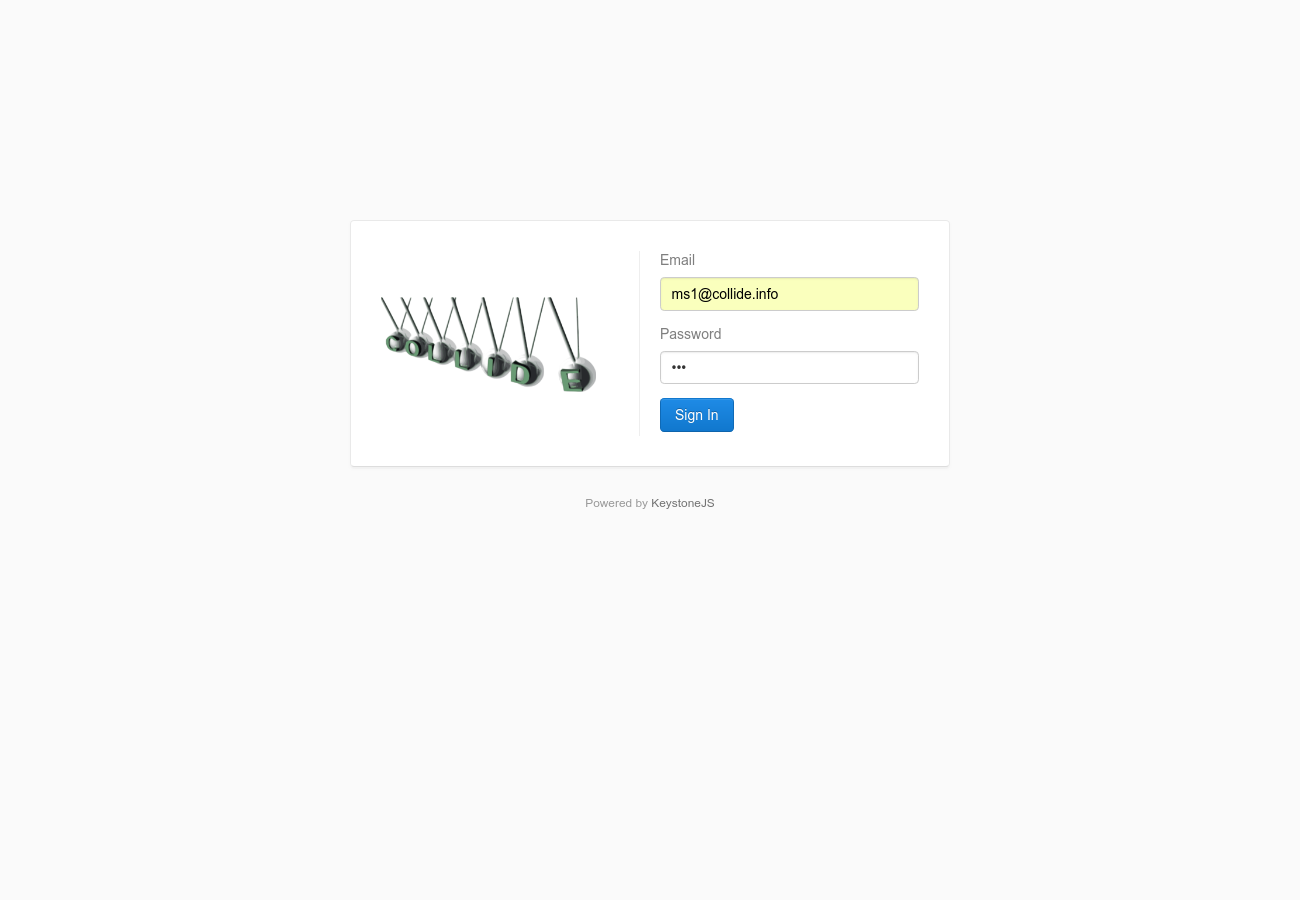
\includegraphics[width=15cm, height=10cm, keepaspectratio]{figures/1-login.png}
  \caption{Der Login-Dialog}
\end{figure}

\begin{figure}
  \centering
  \label{main-menu}
  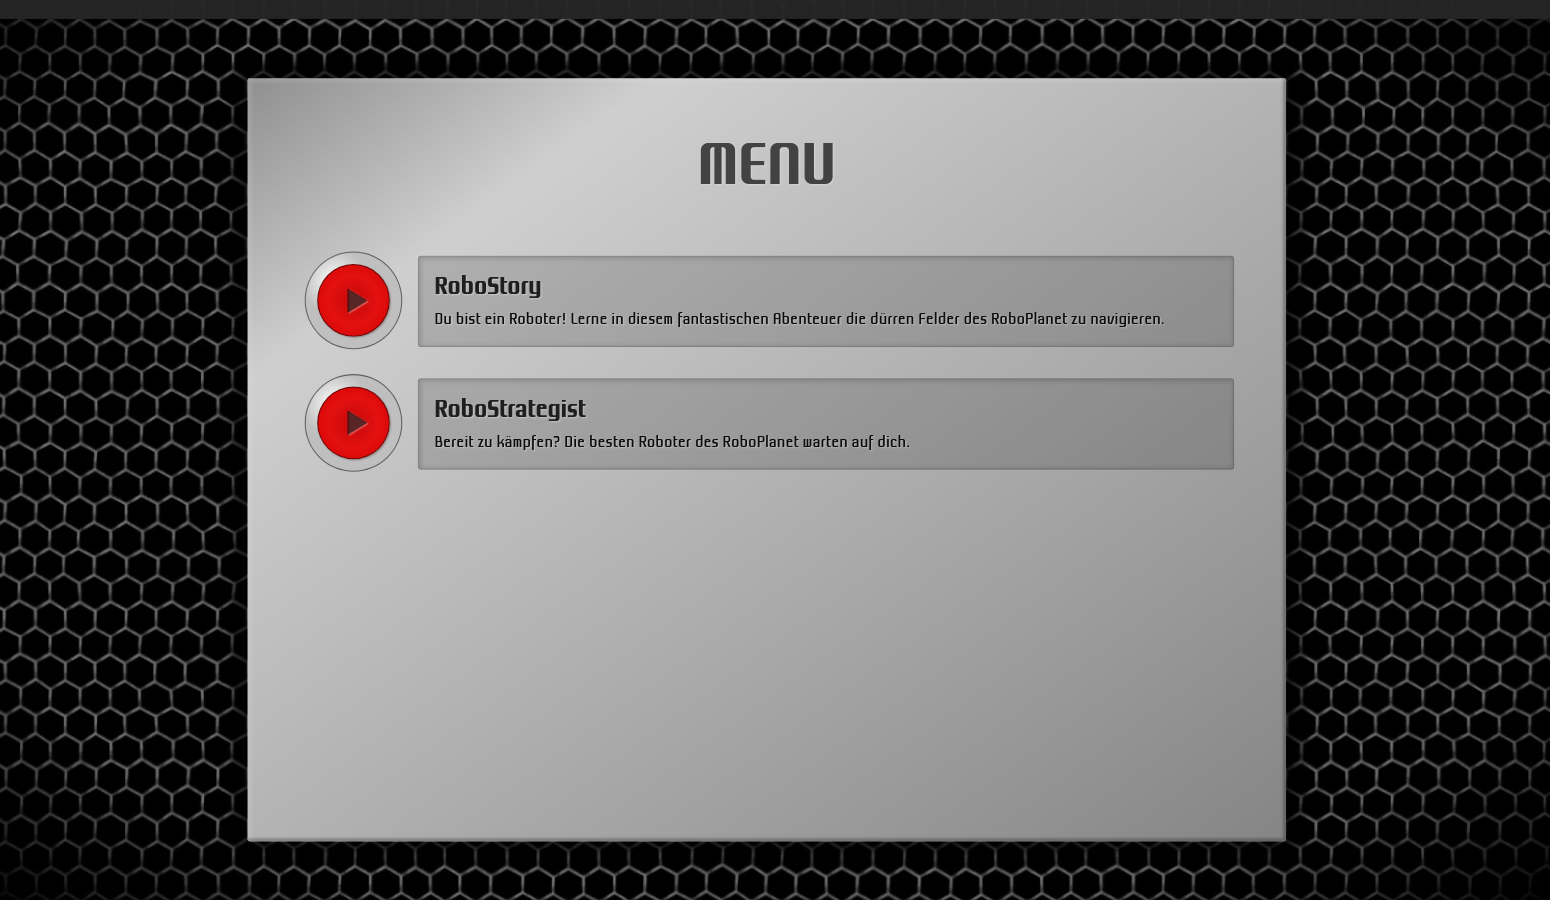
\includegraphics[width=15cm, keepaspectratio]{figures/2-main-menu.png}
  \caption{Das Hauptmenü}
\end{figure}

\begin{figure}
  \centering
  \label{openstage-menu}
  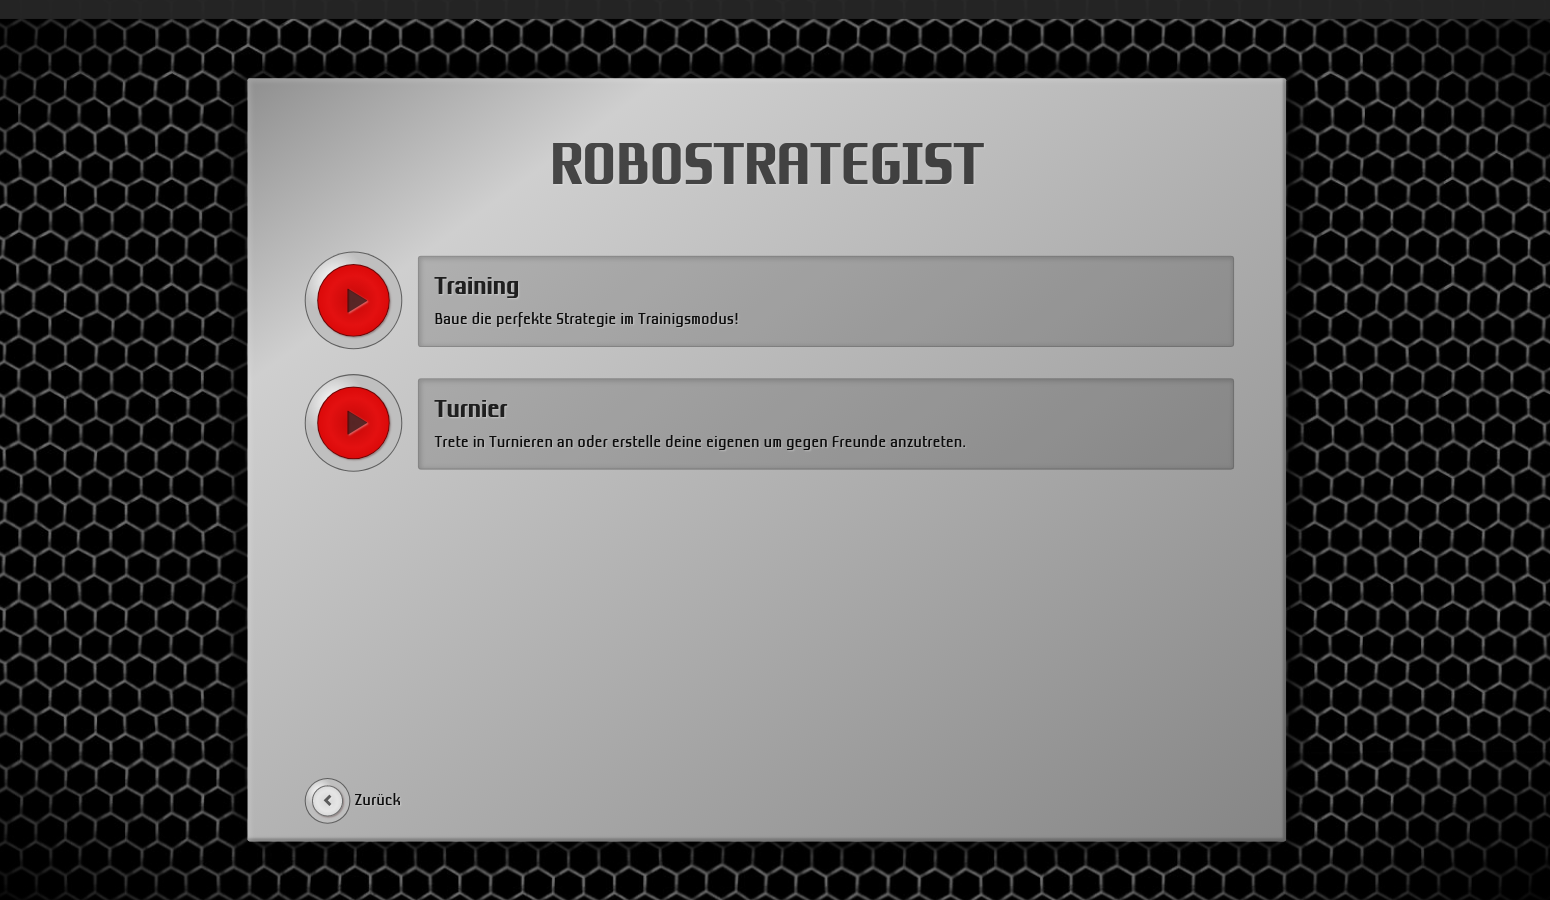
\includegraphics[width=15cm, keepaspectratio]{figures/3-robostrategist-menu.png}
  \caption{Menü des Open Stage-Modus}
\end{figure}

\begin{figure}
  \centering
  \label{training}
  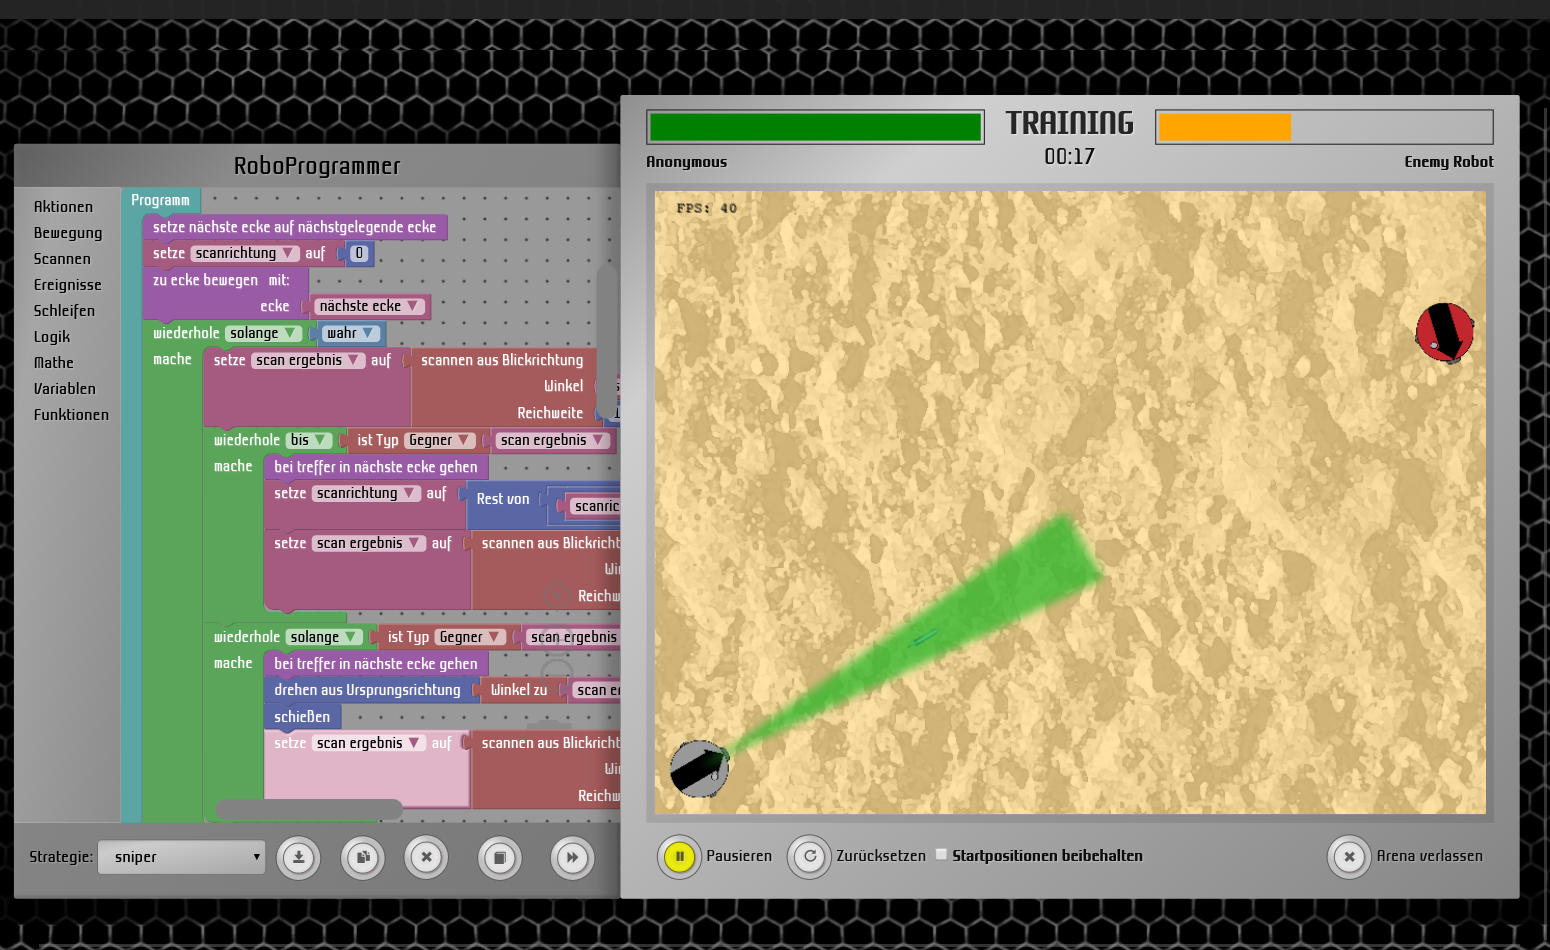
\includegraphics[width=15cm, keepaspectratio]{figures/3-training.png}
  \caption{Die Benutzeroberfläche des Trainings}
\end{figure}

\begin{figure}
  \centering
  \label{training-expanded}
  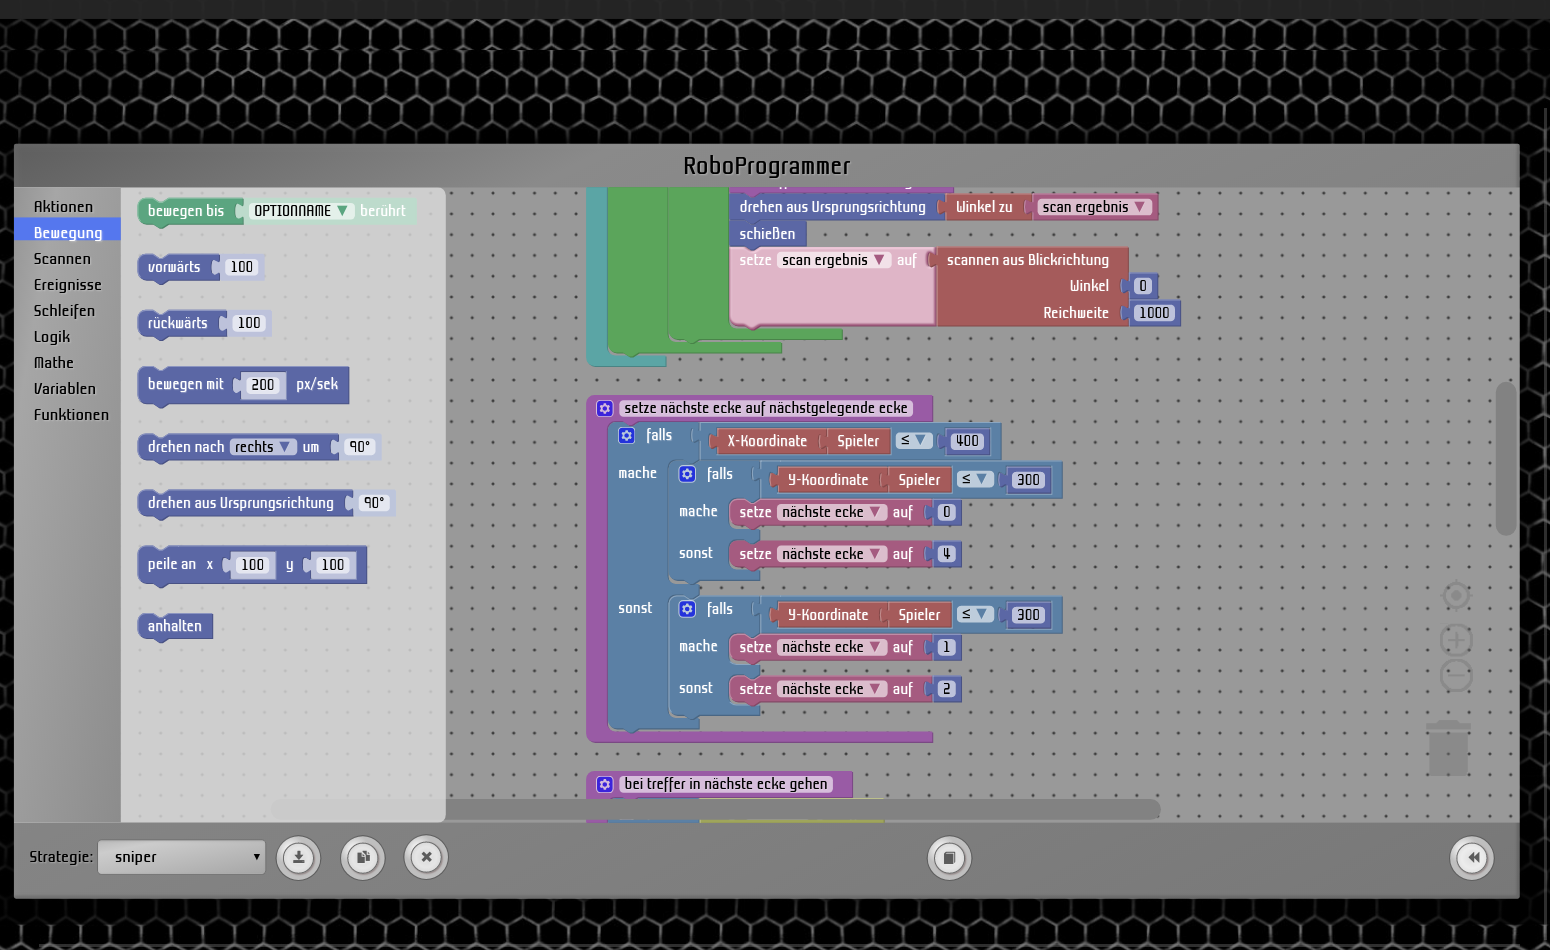
\includegraphics[width=15cm, keepaspectratio]{figures/4-training-expanded.png}
  \caption{Der Strategieeditor im expandiertem Zustand}
\end{figure}

\begin{figure}
  \centering
  \label{tournament-menu}
  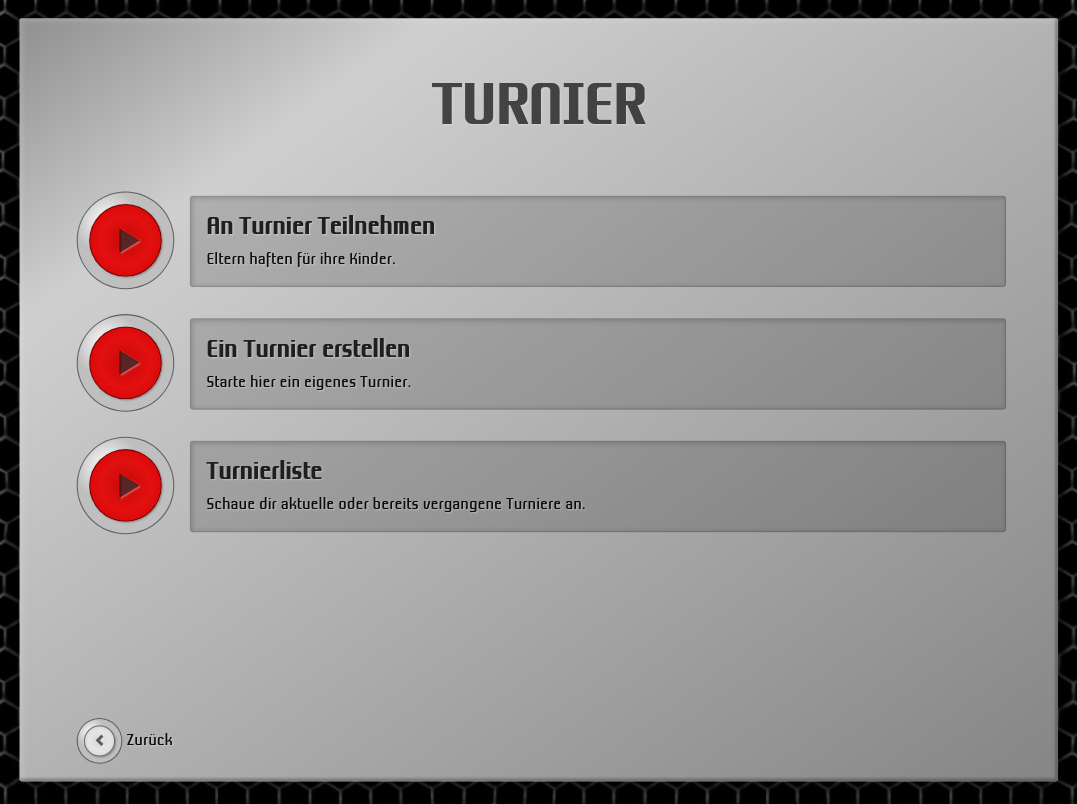
\includegraphics[width=15cm, keepaspectratio]{figures/5-turniermenu.png}
  \caption{Das Turniermenü}
\end{figure}

\begin{figure}
  \centering
  \label{create-tournament}
  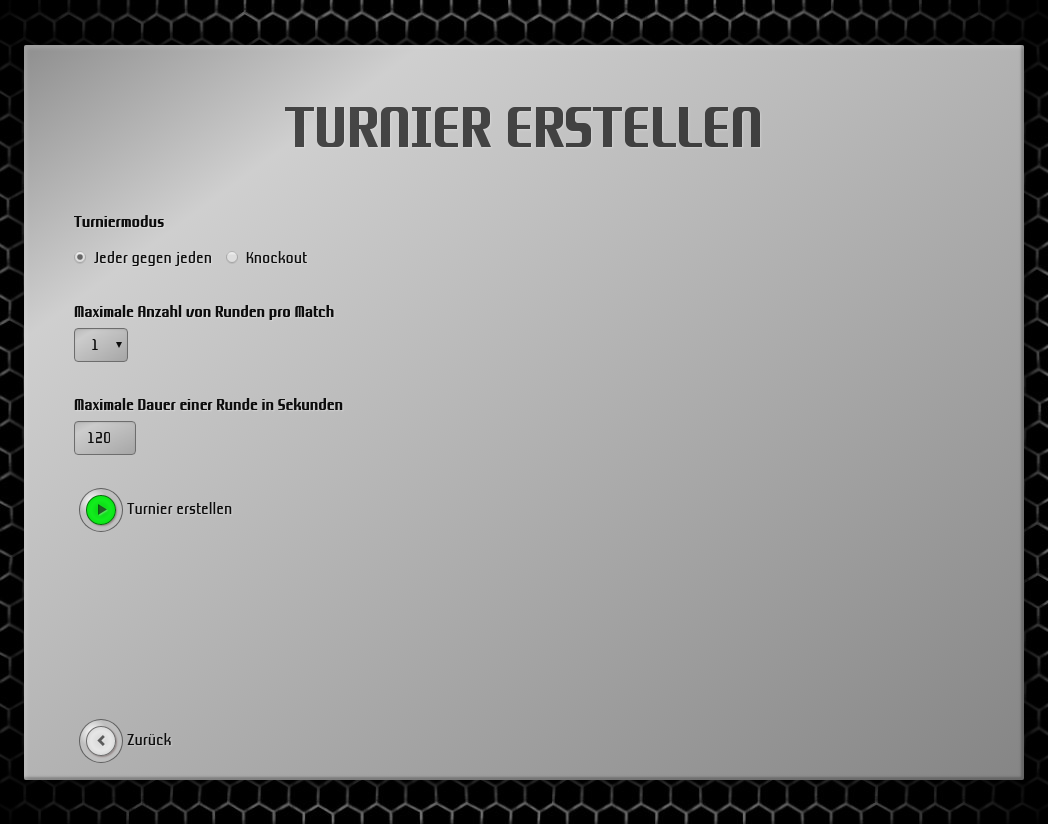
\includegraphics[width=15cm, keepaspectratio]{figures/6-turnier-erstellen-jgj.png}
  \caption{Der Dialog zum Erstellen des Turniers}
\end{figure}

\begin{figure}
  \centering
  \label{create-tournment-code}
  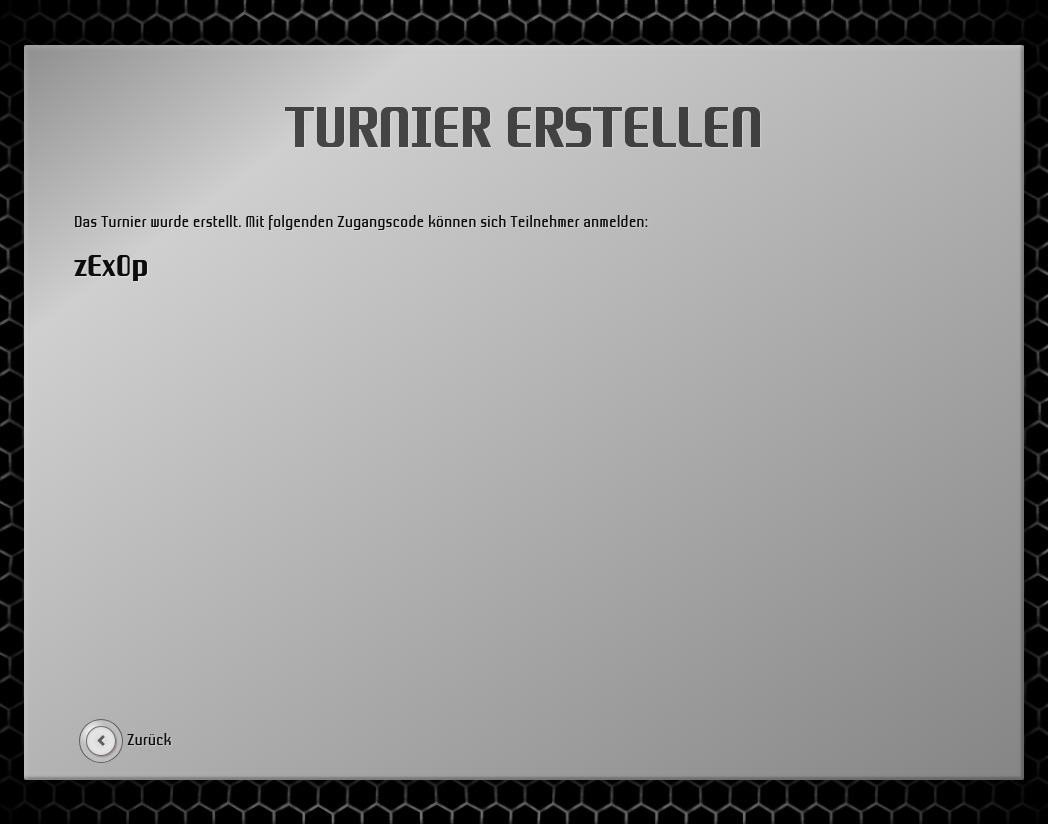
\includegraphics[width=15cm, keepaspectratio]{figures/7-turnier-erstellen-code.png}
  \caption{Der Zugangscode zum Turnier nach Erstellung des Turniers}
\end{figure}

\begin{figure}
  \centering
  \label{participate-tournament}
  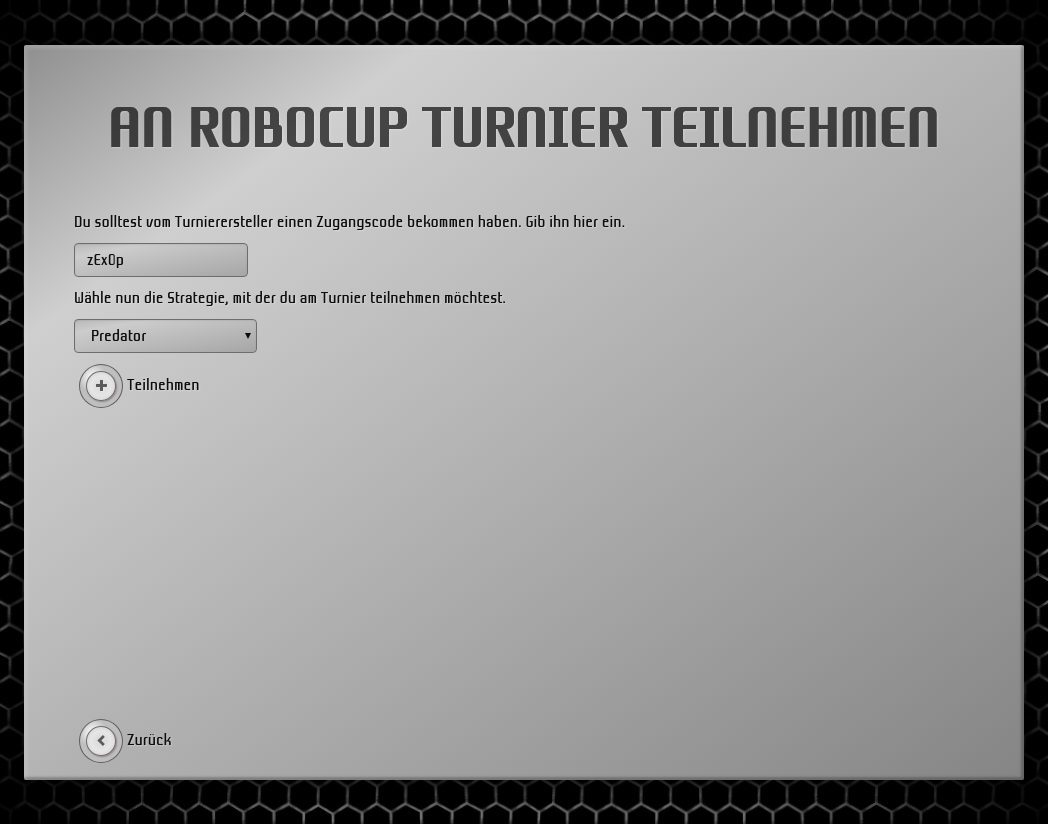
\includegraphics[width=15cm, keepaspectratio]{figures/9-turnierteilnahme.png}
  \caption{Der Dialog zur Teilnahme am Turnier}
\end{figure}

\begin{figure}
  \centering
  \label{tournament-lobby}
  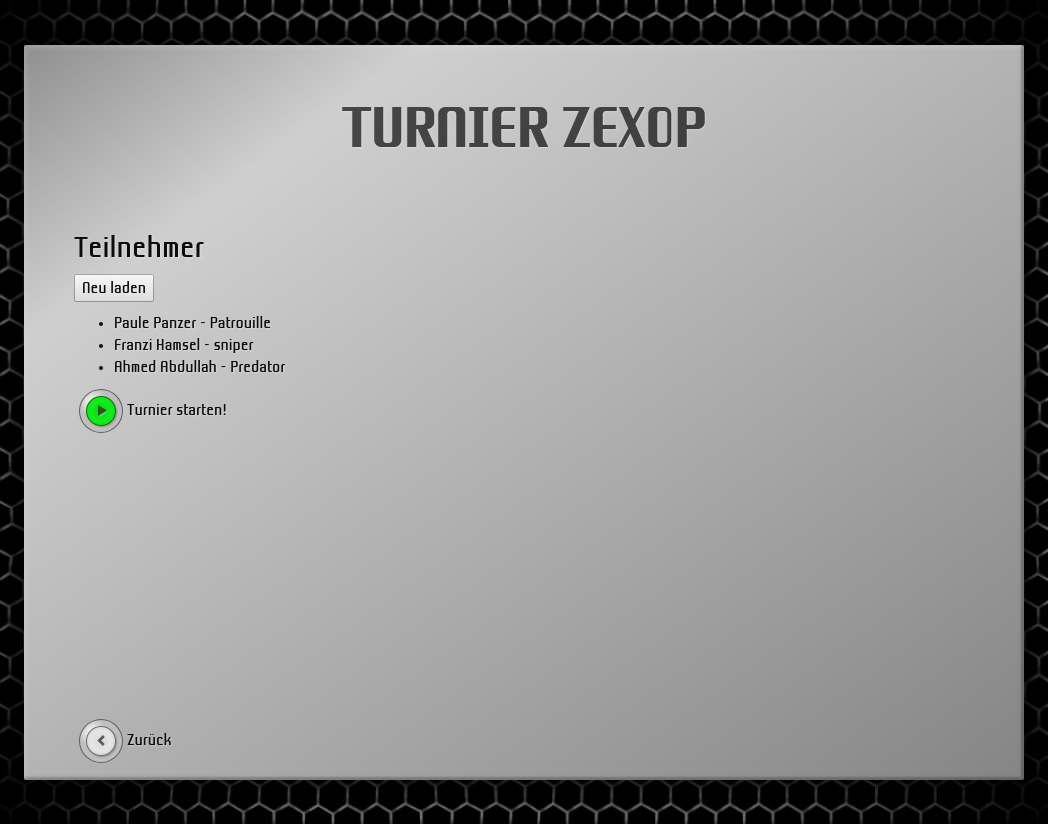
\includegraphics[width=15cm, keepaspectratio]{figures/10-turnierlobby.png}
  \caption{Die Turnierlobby}
\end{figure}

\begin{figure}
  \centering
  \label{tournament-execution-start}
  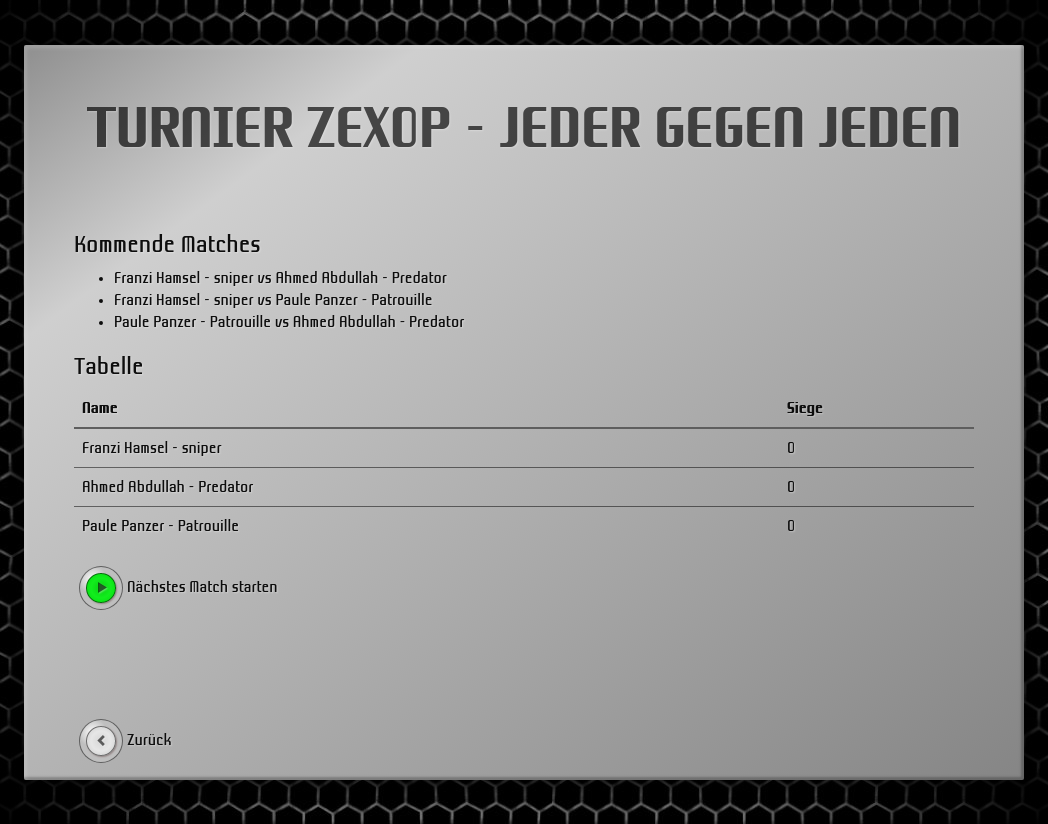
\includegraphics[width=15cm, keepaspectratio]{figures/11-turnierdurchfuehrung-start.png}
  \caption{Die Übersicht zur Turnierdurchführung im Jeder-gegen-Jeden-System zu Beginn eines Turniers}
\end{figure}

\begin{figure}
  \centering
  \label{tournament-execution-match}
  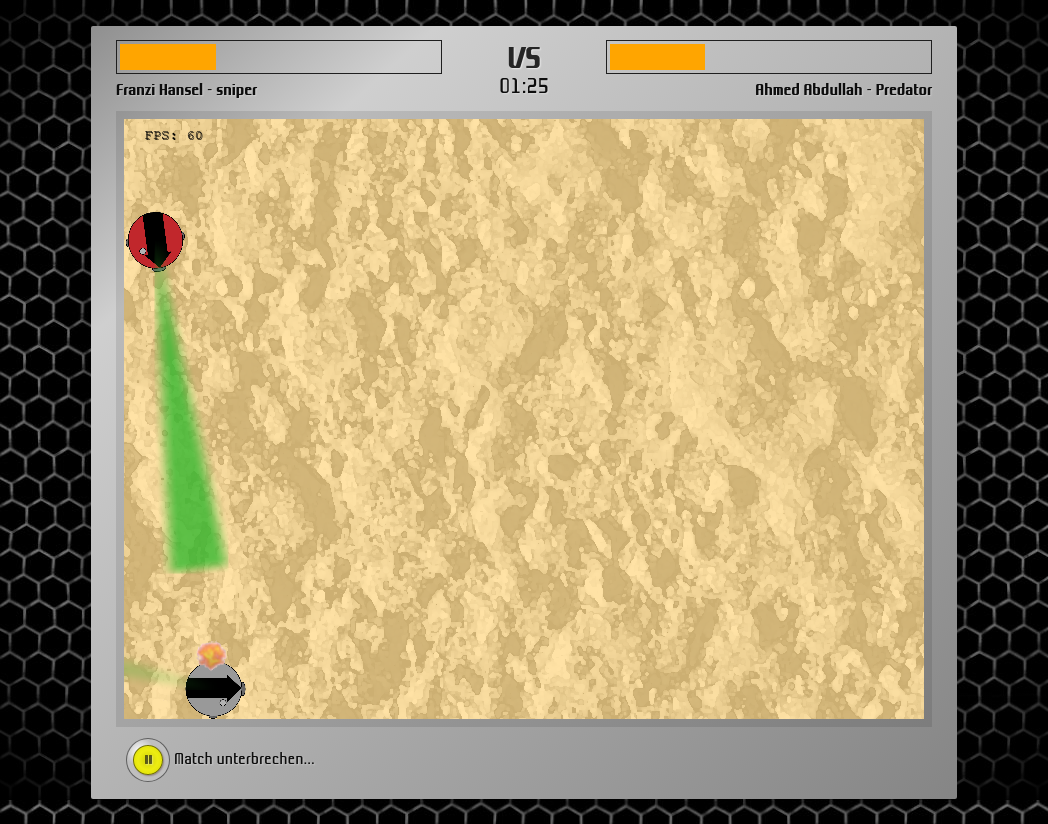
\includegraphics[width=15cm, keepaspectratio]{figures/14-turnierdurchfuehrung-kampf.png}
  \caption{Die Ansicht eines Turnierkampfes}
\end{figure}

\begin{figure}
  \centering
  \label{tournament-execution-mid}
  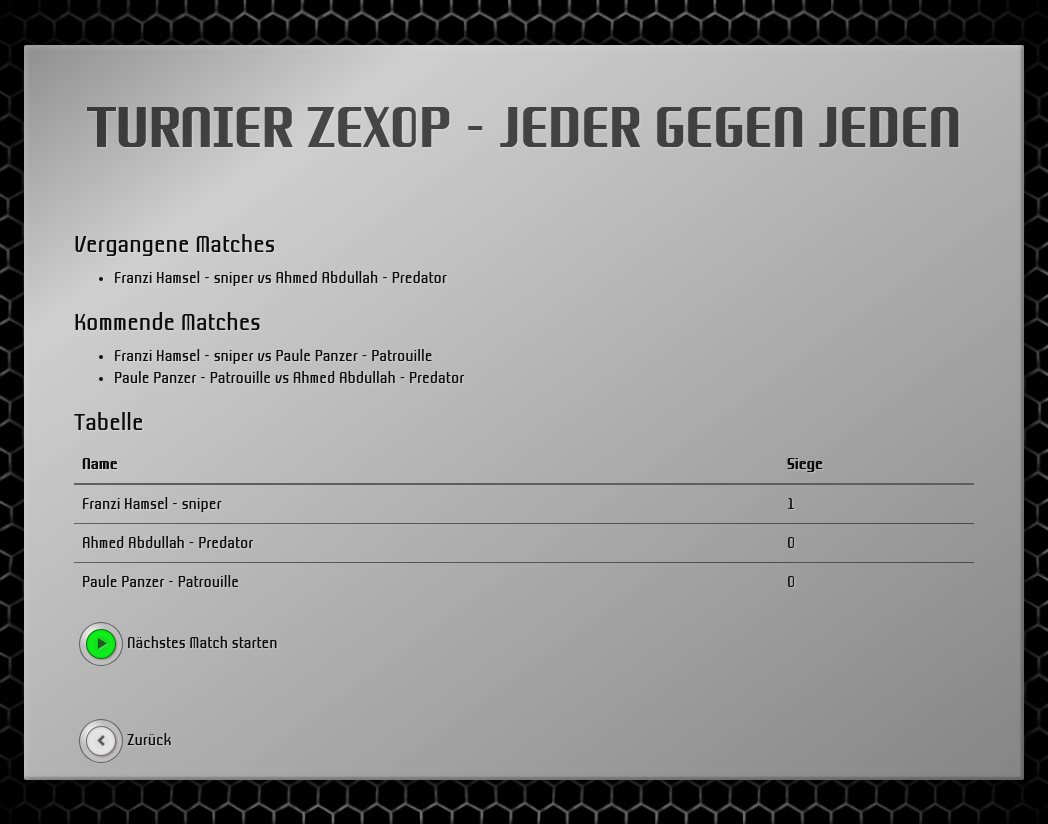
\includegraphics[width=15cm, keepaspectratio]{figures/13-turnierdurchfuehrung-mitte.png}
  \caption{Die Übersicht zur Turnierdurchführung im Jeder-gegen-Jeden-System nachdem ein Kampf durchgeführt wurde}
\end{figure}

\begin{figure}
  \centering
  \label{tournament-execution-end}
  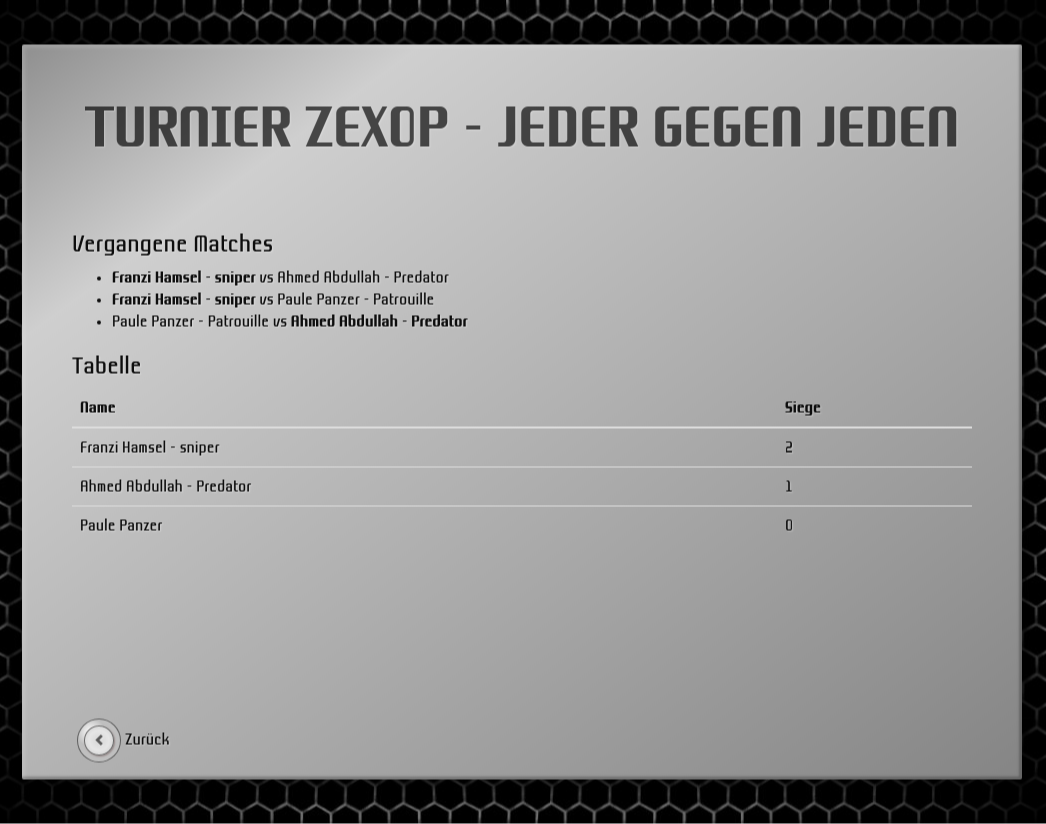
\includegraphics[width=15cm, keepaspectratio]{figures/15-turnierdurchfuehrung-ende.png}
  \caption{Die Übersicht zur Turnierdurchführung im Jeder-gegen-Jeden-System nach Ende des letzten Kampfes}
\end{figure}

\begin{figure}
  \centering
  \label{tournament-execution-ko-start}
  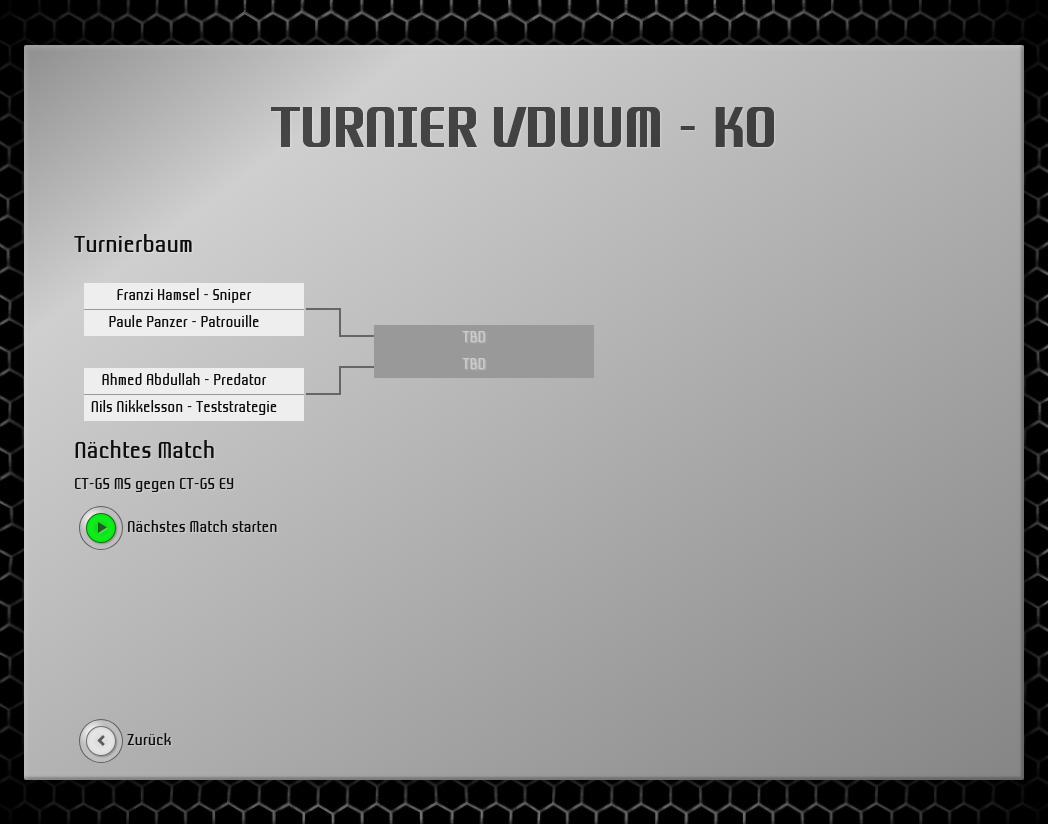
\includegraphics[width=15cm, keepaspectratio]{figures/16-turnierdurchfuehrung-ko-start.png}
  \caption{Die Übersicht zur Turnierdurchführung im KO-System bei Beginn des Turniers}
\end{figure}

\begin{figure}
  \centering
  \label{tournament-execution-ko-start}
  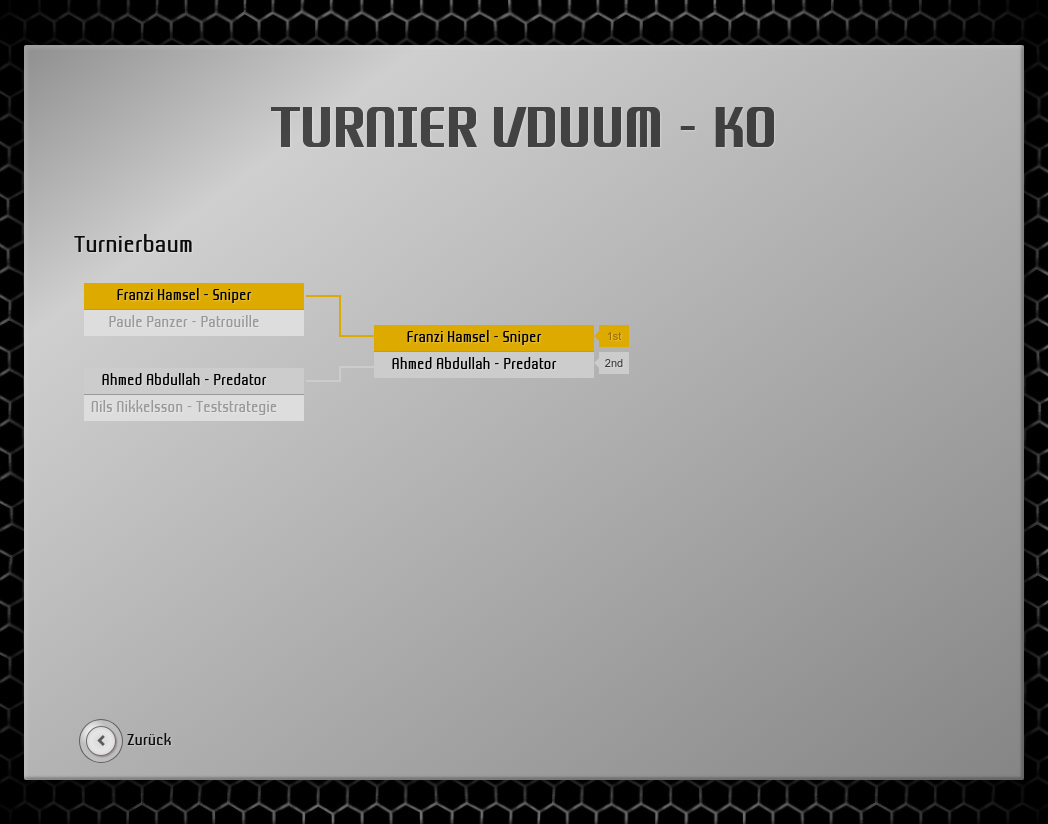
\includegraphics[width=15cm, keepaspectratio]{figures/16-turnierdurchfuehrung-ko-ende.png}
  \caption{Die Übersicht zur Turnierdurchführung im KO-System zum Ende des Turniers}
\end{figure}

\chapter{Evaluation}

\chapter{Zusammenfassung und Ausblick}



% Appendix chapters to be put here. They will be enumerated with capital letters 
% if you  did not change the \documentclass options.
\begin{appendix}
%\include{appendix_chapterA}
\end{appendix}
%Ende Anhang

%Bibliography
% We strongly recommend to use bibtex to manage your bibliography. It helps you
% structure your references and helps avoiding missing important data for a correct
% quotation. If you have no other idea jabref (http://jabref.sourceforge.net/)
% might be a good idea (Jave runtime environment needed).
% This style is good to use in german master thesis'. You need to have activated
% \usepackage{bigerm} above.
% For english documents just use apalike.
%\bibliographystyle{geralpha}

\bibliographystyle{apalike}
% to finally announce where your bibliography is stored use
\bibliography{references}
% it is also possible to have several files separated by comma. 
%Bibliographie Angaben mit \bibliography{}

%\printbibliography
\end{document}

%%% Local Variables:
%%% mode: latex
%%% TeX-master: t
%%% End:
